\let\negmedspace\undefined
\let\negthickspace\undefined
\documentclass[journal, article]{IEEEtran}
\usepackage[a5paper, margin=10mm, onecolumn]{geometry}
\usepackage{lmodern} % Ensure lmodern is loaded for pdflatex
\usepackage{tfrupee} % Include tfrupee package

\setlength{\headheight}{1cm} % Set the height of the header box
\setlength{\headsep}{0mm}     % Set the distance between the header box and the top of the text

\usepackage{lipsum}
\usepackage{tikz}
\usepackage{gvv-book}
\usepackage{gvv}
\usepackage{cite}
\usepackage{amsmath,amssymb,amsfonts,amsthm}
\usepackage{algorithmic}
\usepackage{graphicx}
\usepackage{textcomp}
\usepackage{xcolor}
\usepackage{txfonts}
\usepackage{listings}
\usepackage{enumitem}
\usepackage{mathtools}
\usepackage{gensymb}
\usepackage{comment}
\usepackage[breaklinks=true]{hyperref}
\usepackage{tkz-euclide} 
\usepackage{listings}
\usepackage{gvv}                                        
\def\inputGnumericTable{}                                 
\usepackage[latin1]{inputenc}                                
\usepackage{color}                                            
\usepackage{array}                                            
\usepackage{longtable}                                       
\usepackage{calc}                                             
\usepackage{multirow}                                         
\usepackage{hhline}                                           
\usepackage{ifthen}                                           
\usepackage{lscape}
\usetikzlibrary{matrix, calc}
\begin{document}

\bibliographystyle{IEEEtran}
\vspace{3cm}

\title{10.4.3.8}
\author{EE24BTECH11003 - Akshara Sarma Chennubhatla}
% \maketitle
% \newpage
% \bigskip
{\let\newpage\relax\maketitle}
\textbf{Question:}
A train travels $360km$ at a uniform speed. If the speed had been $5km/h$ more, it would have taken $1$ hour less for the same journey. Find the speed of the train.

\solution\\
\textbf{Theoretical Solution:}\\

Let $s$ be the speed of the train, then,
\begin{align}
	\frac{360}{s} - 1 &= \frac{360}{s + 5}\\
	\implies s^2 + 5s &= 1800
\end{align}
This is a quadratic equation whose roots are the possible values of the speed.\\
Using the quadratic formula,
\begin{align}
	s &= \frac{-5 \pm \sqrt{5^2 - 4\brak{1}\brak{-1800}}}{2\brak{1}}\\
	s &= -45, 40
\end{align}

\textbf{Simulated Solution:}\\

\textbf{By Newton-Ralphson method,}\\
Take initial guess $s_0$, then run the following loop,
\begin{align}
	s_{n+1} &= s_n - \frac{f\brak{s_n}}{f^\prime\brak{s_n}}\\
	f\brak{s} &= s^2 + 5s - 1800\\
	f^\prime\brak{s} &= 2s + 5\\
	s_{n+1} &= s_n - \frac{s_n^2 + 5s_n - 1800}{2s_n + 5}
\end{align}
This method converges for real roots but when roots are complex, it can go to infinity as well. To avoid that, if our roots are complex, take initial guess as a complex number.
The values of $s$ got through this method are,
\begin{align}
	s &= -45\\
	s &= 40
\end{align}

Alternatively, we can solve the question by using the eigen values of the companion matrix.\\
For a polynomial equation of form $x_n+c_{n-1}x^{n-1}+\dots+c_2x^2+c_1x+c_0 = 0$ the companion matrix if of the form
\begin{align}
	\myvec{
		0 & 0 & \cdots & 0 & -c_0\\
		1 & 0 & \cdots & 0 & -c_1\\
		0 & 1 & \cdots & 0 & -c_2\\
		\vdots & \vdots & \ddots & \vdots & \vdots\\
		0 & 0 & \cdots & 1 & -c_{n-1}\\
	}
\end{align}
The eigen values of this matrix are the roots of the polynomial equation. For this question,
\begin{align}
	n &= 2\\
	c_0 &= -1800\\
	c_1 &= 5\\
	C &= \myvec{0 & 1800 \\ 1 & -5}
\end{align}
To find the eigen values of the matrix, we use the method of QR decomposition of the matrix.\\
The QR algorithm decomposes a matrix A into the product of an orthogonal matrix Q and an upper triangular matrix R, such that
\begin{align}
	A = QR
\end{align}
The matrix is then updated iteratively as:
\begin{align}
	A_{new} = RQ
\end{align}
This process is repeated until A converges to an upper triangular form.\\
Steps to perform QR decomposition with accelerated convergence,\\
\begin{enumerate}
	\item \text{Convert to Upper Hessenberg form via Householder Reflections}
	\item \text{Performing QR decomposition via Givens Rotations with shifts}
	\item \text{Read off diagonal elements}
\end{enumerate}
\textbf{Householder Reflections:}\\
A square matrix A of order $n \times n$ is said to be in upper Hessenberg form if all the entries below the first subdiagonal are zero.
For example:
\begin{align}
	H = 
	\begin{bmatrix}
		h_{11} & h_{12} & h_{13} & \cdots & h_{1n} \\
		h_{21} & h_{22} & h_{23} & \cdots & h_{2n} \\
		0      & h_{32} & h_{33} & \cdots & h_{3n} \\
		\vdots & \ddots & \ddots & \ddots & \vdots \\
		0      & \cdots & 0      & h_{n-1,n-1} & h_{n-1,n} \\
		0      & \cdots & \cdots & 0          & h_{nn} \\
	\end{bmatrix}
\end{align}
\begin{enumerate}
	\item Select a Subvector $\vec{x}$:
\begin{align}
	x = \begin{bmatrix}
		A_{2,1} \\
		A_{3,1} \\
		\vdots \\
		A_{n,1}
	\end{bmatrix}.
\end{align}

\item Define the Target Vector:
	The goal is to transform $\vec{x}$ into a new vector $\vec{y}$ where only the first element is non-zero, and all the other elements are zero. First, compute $\norm{x}$:

		\begin{align}
			\vec{y} = \pm \norm{x} e_1,
		\end{align}

\item Construct the Householder Vector $\vec{v}$:
	To generate a reflection that transforms \( x \) to \( y \), the Householder vector \( v \) is defined as:

		\begin{align}
			v &= x - \text{sign}(x_1) \norm{x} e_1\\
			\text{sign}(x_1) &= \frac{x_1}{|x_1|},
		\end{align}

	After defining \( v \), it is normalized to a unit vector:

\item Construct the Householder Matrix \( H_k \):
	The Householder matrix \( H_k \) is constructed as:

		\begin{align}
		H_k = I - 2 \frac{v v^*}{v^* v},
		\end{align}

\item Apply the Householder Transformation:
	The matrix \( H_k \) is applied to \( A \) as:

		\begin{align}
		A' = H_k A H_k^*,
		\end{align}

	This will reduce the matrix to Hessenberg form by eliminating the sub-diagonal elements of the first column.

\item Repeat for Subsequent Columns:
	This Householder transformation approach ensures that the matrix is gradually transformed to a Hessenberg form, where all elements below the first sub-diagonal are zero.
\end{enumerate}

\newpage
\textbf{Givens Rotations:}

\begin{center}
\begin{tikzpicture}
  % Original Hessenberg Matrix
  \matrix[matrix of math nodes, left delimiter={[}, right delimiter={]}] (hessenberg) {
    h_{11} & h_{12} & h_{13} & \cdots & h_{1n} \\
    h_{21} & h_{22} & h_{23} & \cdots & h_{2n} \\
    0      & h_{32} & h_{33} & \cdots & h_{3n} \\
    \vdots & \ddots & \ddots & \ddots & \vdots \\
    0      & \cdots & 0      & h_{n-1,n-1} & h_{n-1,n} \\
    0      & \cdots & \cdots & 0          & h_{nn} \\
  };

  % Arrow indicating Givens rotation
  \node[above of=hessenberg, yshift=-3cm] (arrow) {\(\longrightarrow\)};
  
  % Upper Triangular Matrix after QR
  \matrix[matrix of math nodes, left delimiter={[}, right delimiter={]}, right of=arrow, xshift=6cm] (upper) {
    r_{11} & r_{12} & r_{13} & \cdots & r_{1n} \\
    0      & r_{22} & r_{23} & \cdots & r_{2n} \\
    0      & 0      & r_{33} & \cdots & r_{3n} \\
    \vdots & \ddots & \ddots & \ddots & \vdots \\
    0      & \cdots & 0      & r_{n-1,n-1} & r_{n-1,n} \\
    0      & \cdots & \cdots & 0          & r_{nn} \\
  };

  % Arrows to show step-by-step elimination
  \draw[->, thick] (hessenberg-2-1) -- (upper-2-1);
  \draw[->, thick] (hessenberg-3-2) -- (upper-3-2);
  \draw[->, thick] (hessenberg-4-3) -- (upper-4-3);
\end{tikzpicture}
\end{center}

Each Givens rotation zeros out a specific subdiagonal element, progressively transforming the Hessenberg matrix into an upper triangular matrix.

	To choose the values of $c$ and $s$ for the Givens rotation in QR decomposition, let $a_j$ be the element we wish to null out (i.e. make 0). Pick an arbitrary non-zero pivot element $a_i$ (on a different row). Usually, if we wish to null a particular sub-diagonal element, we pick the principal diagonal element above it as a pivot.
	\begin{align}
		c = \frac{\overline{a_{i}}}{\sqrt{a_{i}^2 + a_{j}^2}}, \quad s = \frac{-\overline{a_{j}}}{\sqrt{a_{i}^2 + a_{j}^2}}
	\end{align}
	Givens rotation essentially rotates the two rows that $a_i$ and $a_j$ are on such that $a_j = 0$ after rotation, other rows remain unaffected.\\ 

	Visualizing the process,
	\begin{align}
		\begin{bmatrix}
			\times & \times & \times & \times \\
			\times & \times & \times & \times \\
			0 & \times & \times & \times \\
			0 & 0 & \times & \times
		\end{bmatrix}
		\xrightarrow{G(3,2,\theta_1)}
		\begin{bmatrix}
			\times & \times & \times & \times \\
			\times & \times & \times & \times \\
			0 & 0 & \times & \times \\
			0 & 0 & \times & \times
		\end{bmatrix}
		\xrightarrow{G(4,3,\theta_2)}
		\begin{bmatrix}
			\times & \times & \times & \times \\
			\times & \times & \times & \times \\
			0 & 0 & \times & \times \\
			0 & 0 & 0 & \times
		\end{bmatrix}.
	\end{align}
	After all Givens rotations, the resulting matrix is upper triangular:
	\begin{align}
		R = \begin{bmatrix}
			\times & \times & \times & \times \\
			0 & \times & \times & \times \\
			0 & 0 & \times & \times \\
			0 & 0 & 0 & \times
		\end{bmatrix}.
	\end{align}

	The sequence of Givens rotations $G_1, G_2, \dots, G_m$ satisfies:
	\begin{align}
		G_m \cdots G_2 G_1 A = R,
	\end{align}
	where \(R\) is upper triangular. The QR decomposition is obtained by combining the transposes of the Givens rotations into \(Q\):
	\begin{align}
		A = Q R, \quad Q = G_1^{\top} G_2^{\top} \cdots G_m^{\top}.
	\end{align}
	\begin{align}
		A_{k+1}&= R_k Q_k\\
		&=(G_n \dots G_2 G_1)A_k(G_1^{\top}G_2^{\top}\dots G_n^{\top})\\
		&= (G_n \dots G_2 G_1)A_k(G_n \dots G_2 G_1)^{\top}
	\end{align}
	Iteratively repeating this process causes the matrix to converge to upper triangular.\\

\textbf{Handling Jordan Blocks:}\\
Jordan blocks pose challenges in eigenvalue computation because the matrix cannot be diagonalized. A Jordan block for eigenvalue \(\lambda\) appears as:

\begin{align}
\begin{bmatrix}
a & b \\
c & d
\end{bmatrix}
\end{align}

where a and b are the diagonal elements and c is a non zero sub-diagonal element.\\
To handle Jordan blocks, the QR algorithm implemented here solves for the eigenvalues directly using the characteristic polynomial of the block. For a \(2 \times 2\) Jordan block, the eigenvalues are roots of:

\begin{align}
\lambda^2 - (\text{trace})\lambda + \det = 0.
\end{align}

In this case, the eigen values of the matrix computed are,
\begin{align}
	\lambda_1 = -45\\
	\lambda_2 = 40\\
\end{align}

Below is the plot for given quadratic equation, obtained by iterating through the values of $x$ with step size of $h$
	\begin{figure}[h!]
		\centering
		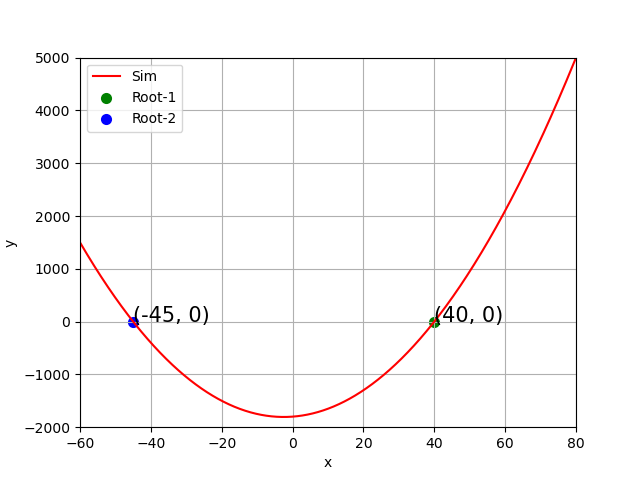
\includegraphics[width=1\columnwidth]{figs/simulated.png}
		\caption{Plot of $s^2 + 5s = 1800$}
		\label{stemplot}
	\end{figure}

\end{document}
